\section{Namespace: GUI Laget}

\begin{figure}[H]
	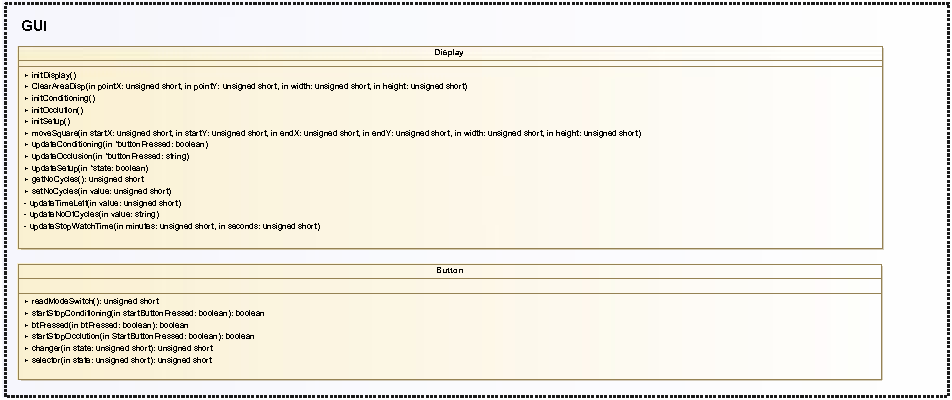
\includegraphics[width=\textwidth]{klassediagram_GUI-crop.pdf}
	\caption{Klasse diagram over namespacet GUI}\label{fig:classDiagramGUI}
\end{figure}

\subsection{Klasse: Display}
Denne klasse gør brug af to biblioteker for at kunne bruge TFT skærmen, henholdvis Adafruit\_GFX og Adafruit\_ILI9340. For at kunne kommunikere med displayet gøre der brug af disse bibliotekters indbyggede funktioner. Derfor oprettes et objekt af klassen Adafruit\_ILI9340 kaldet TFTscreen.

\subsubsection{Metode: initDisplay()}
\textbf{Parameter: } \textit{void}
\\ \textbf{Returtype: } \textit{void}
\\ \textbf{Beskrivelse: } Her initieres skærmen med funktion \textit{.begin().} Rotationen og baggrundsfarven af skærmen sættes også når denne metode kaldes. Skærmrotationen er sat 3, hvilken betyder at skærmen er i “landscape mode”. 

\subsubsection{Metode: clearAreaDisp()}
\textbf{Parameter: } \textit{unsigned short pointX, unsigned short pointY, unsigned short width, unsigned short height}
\\ \textbf{Returtype: } \textit{void}
\\ \textbf{Beskrivelse: } Da skærmen baggrundsfarven er sat til sort, medtager denne metode 4 parameter hhv. start x-koordinat, start y-koordinat, bredde og højde. Disse parameter fortæller hvor og hvor en del af skærmen der skal farves sort, og dermed slette det område.

\subsubsection{Metode: initConditioning()}
\textbf{Parameter: } \textit{void}
\\ \textbf{Returtype: } \textit{void}
\\ \textbf{Beskrivelse: } Når denne metode kaldes skrives de “faste” værdier på skærmen til et konditioneringsforløb. På billedet nedenfor ses hvordan skærmen ser ud, når metoden er kørt. Et eksempel på hvordan der skrives tekst på skærmen: 
\begin{lstlisting}
TFTscreen.setTextColor(ILI9340_WHITE);  TFTscreen.setTextSize(2);
TFTscreen.setCursor(0, 0);
TFTscreen.println("ID: ");
\end{lstlisting}
Først fortælles hvilken farve teksten skal have, dernæst tekststørrelse og placering. Til sidst angives hvilken tekst der skal printes på skærmen

\begin{figure}[H]
	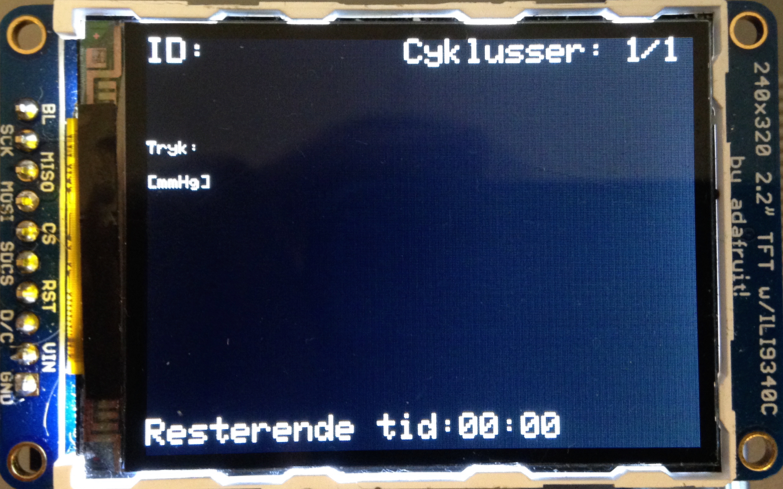
\includegraphics[width=\textwidth]{billeder/conditioning.png}
	\caption{Eksempel på layout når initConditioning() bliver kaldt}\label{pic:conditiong}
\end{figure}

\subsubsection{Metode: initOcclusion()}
\textbf{Parameter: } \textit{void}
\\ \textbf{Returtype: } \textit{void}
\\ \textbf{Beskrivelse: }  Denne metode bruges til at opsætte skærmen for okklusionstræningsforløb. Der skrives tid og enheden for tryk på skærmen. Se billedet nedenfor for layoutet. 

\begin{figure}[H]
	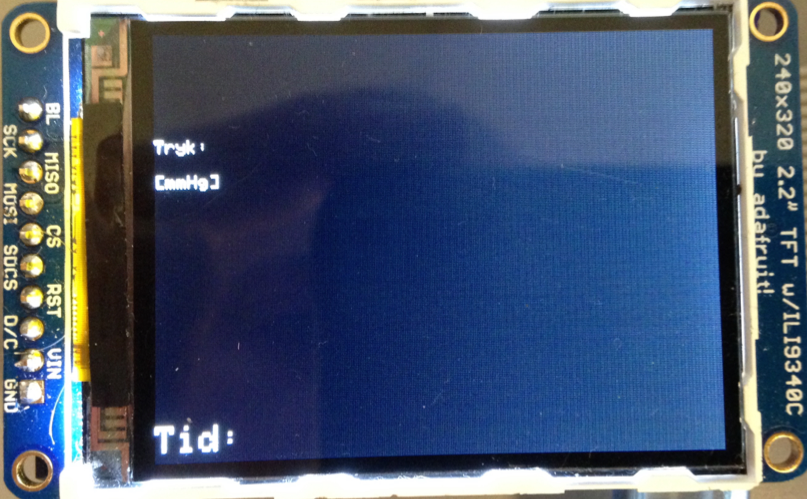
\includegraphics[width=\textwidth]{billeder/occlusion.png}
	\caption{Eksempel på layout når initOcclusion() bliver kaldt}\label{pic:occlusion}
\end{figure}

\subsubsection{Metode: initSetup()}
\textbf{Parameter: } \textit{void}
\\ \textbf{Returtype: } \textit{void}
\\ \textbf{Beskrivelse: } Her opsættes skærmen for setup programmet. Teksten “\textit{Tid pr cyklus}” og “\textit{Antal cyklusser}” er faste værdi på skærmen. Men værdierne hentes fra logik laget, så de er opdateret. 

\begin{figure}[H]
	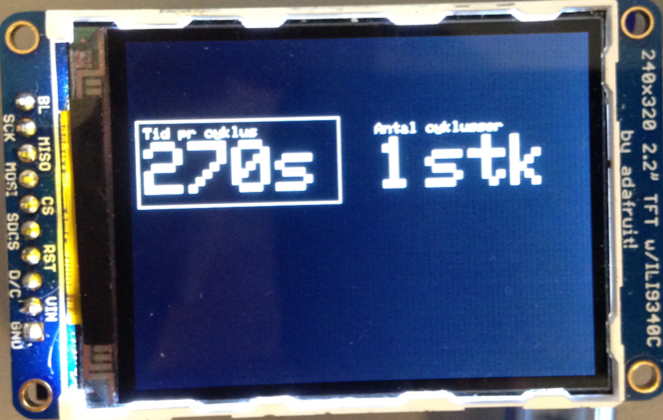
\includegraphics[width=\textwidth]{billeder/setup.png}
	\caption{Eksempel på layout når initSetup() bliver kaldt}\label{pic:setup}
\end{figure}

\subsubsection{Metode: moveSquare()}
\textbf{Parameter: } \textit{unsigned short startX, unsigned short startY, unsigned short endX, unsigned short endY, unsigned short width, unsigned short height}
\\ \textbf{Returtype: } \textit{void}
\\ \textbf{Beskrivelse: } Denne metode bruges til at flytte cursoren på skærmen under setup. For at slette noget på skærmen skal det farves samme farve som baggrunden. Derfor får metoden  x- og y-koordinaterne for den firkant der skal slettes, samt x- og y-koordinaterne for hvor den nye firkant skal tegnes henne. Desuden skal metode også have bredde og højde på firkanten. For at sikre at der ikke kan lavet et interrupt inde i metode, gør metode brug af den indbyggede funktion \textit{noInterrupt()}. Et interrupt på det forkerte tidspunkt ville betyde at skærm ikke ville slette den forrige firkant eller ikke ville tegne det nye. 

\subsubsection{Metode: updateConditioning()}
\textbf{Parameter: } \textit{volatile bool *buttonPressed}
\\ \textbf{Returtype: } \textit{void}
\\ \textbf{Beskrivelse: } Metoden modtager en pointer, som peger på værdien af \textit{buttonPressed}. Hvis værdien af denne er sand, samt at antallet af kørte cyklusser ikke er lig med nul, vil metoden køre et loop, hvor der ved hjælp af timer klassen fra logik laget bliver starten en nedtælling, så loop vil køre indtil tiden er løbet ud. Mens loopet kører, opdaterer skærmen konstant værdien fra tryksensor og fortæller trykket i manchetten.  Strukturen på metoden ser ud på følgende måde: 
\begin{lstlisting}
	while(*buttonPressed && getNoCycleLeft() !=0){
	if(!timer.getTimerStatus()){
		//Runing conditioning threatment 
	}else
		//Reseting the timer
	}
	if(!*buttonPressed)
		//Handle if the conditioning threatment has ended, and the user want to reset
\end{lstlisting}
Derfor er det værdien af \textit{buttonPressed} og \textit{getNoCycleLeft()} der afgører om loopet eksekveres. Hvis værdien af \textit{buttonPressed} er falsk, så skrives det sidste værdi af timeren og sensorværdien slettes på skærmen.  \\

\textit{buttonPressed} styres ved knaptryk og bruger kan derfor starte og stoppe konditionerings forløbet på denne måde. Hvis forløbet stopper af sig selv, altså hvis antallet af tilbageværende cyklusser er nul, så håndtere metoden af brugeren ikke skal trykke to gange på knappen for at starte et nyt forløb. 
\begin{lstlisting}
	if(memory.getNoOfCycles() == 0)
		*buttonPressed = false;
\end{lstlisting}

\subsubsection{Metode: updateOcclusion()}
\textbf{Parameter: } \textit{volatile bool *buttonPressed}
\\ \textbf{Returtype: } \textit{void}
\\ \textbf{Beskrivelse: } Denne metode køres når der apparatet er sat på okklusions træningsforløb. Denne metode bruger også pointeren til \textit{buttonPressed}, hvis den er true eksekveres et while loop hvor der startes et stopur og trykket fra manchetten vises på skærmen. Hvis værdien er falsk slettes sensorværdien på displayet, og slut tiden vises fra stopuret.

\subsubsection{Metode: updateSetup()}
\textbf{Parameter: } \textit{volatile bool *state}
\\ \textbf{Returtype: } \textit{void}
\\ \textbf{Beskrivelse: } Til styring af cursoren på displayet i setup. Denne metode består af en switch case struktur, som har fire cases og casevalg afgøres af værdien af *state. Case 0 og 1 er gøre brug af metoden \textit{moveSquare(..)} som flytter cursoren. Case 2 og 3 sørge for at vise værdien af hhv tid pr cyklus og antal cyklusser. Da cursoren styres med interrupt er interrupts slået fra så længe koden afvikles inde i case 2 og 3. 

\subsubsection{Metode: getNoCycles()}
\textbf{Parameter: } \textit{void}
\\ \textbf{Returtype: } \textit{unsigned short}
\\ \textbf{Beskrivelse: } Bruges til at hente \textit{antal cyklusser} fra logik laget. Denne værdi aflæses fra EEPROM via data laget, men for at overholde 3-lags modellen skal kommunikation gå via logik laget. 

\subsubsection{Metode: setNoCycles()}
\textbf{Parameter: } \textit{unsigned short value}
\\ \textbf{Returtype: } \textit{void}
\\ \textbf{Beskrivelse: } Bruges til at sætte at værdien af \textit{antal cyklusser}. 

\subsubsection{Metode: updateTimeLeft()}
\textbf{Parameter: } \textit{unsigned short value}
\\ \textbf{Returtype: } \textit{void}
\\ \textbf{Beskrivelse: } Denne metode er lavet til opdate tiden under konditioneringsforløbet. Da det kræver 5 metodekald af metoder fra biblioteket \textit{Adafruit\_ILI9340} for at skrive tekst på skærmen er dette indkapslet i én metode, som blot skal have en String value. 

\subsubsection{Metode: updateNoOfCycles()}
\textbf{Parameter: } \textit{String value}
\\ \textbf{Returtype: } \textit{void}
\\ \textbf{Beskrivelse: } Når metoden kaldes opdateres antallet cyklusser på skærmen. 

\subsubsection{Metode: updateStopWatchTime()}
\textbf{Parameter: } \textit{unsigned short minutes, unsigned short seconds}
\\ \textbf{Returtype: } \textit{void}
\\ \textbf{Beskrivelse: } Denne metode opdatere tiden fra stopuret på displayet under okklusions træningsforløbet 

\subsection{Klasse: Buttons}

\subsubsection{Metode: readModeSwitch()}
\textbf{Parameter: } \textit{void}
\\ \textbf{Returtype: } \textit{unsigned short}
\\ \textbf{Beskrivelse: } Denne metode læser tre digitale pins hhv; 22, 24, og 26. Her vil én pin være høj og de to andre lave. Metoden afgøre ud fra hvilken pin der er høj, om der skal køres hhv; konditioningsforløb, okklusionstræning eller setup. Denne metode bliver kaldt i én gang når arduinoen startes op. Skal der ændres på hvilken forløb apparatet skal køre, skal arduinoen genstartes. 

\subsubsection{Metode: startStopConditioning()}
\textbf{Parameter: } \textit{volatile bool startButtonPressed}
\\ \textbf{Returtype: } \textit{bool}
\\ \textbf{Beskrivelse: } Styring af værdien for \textit{startButtonPressed}. Hver gang metode køres inverteres værdien af \textit{startButtonPressed}. Desuden indeholde metoden et \textit{if/else} statement, der hvis værdien af \textit{startButtonPressed} er falsk sletter den gamle måling på skærmen og resetter antallet af kørte cyklusser. Hvis værdien er sand sættes et tidsstempel, så timeren passer når et nyt forløb startes.  

\subsubsection{Metode: btPressure()}
\textbf{Parameter: } \textit{volatile bool btPressed}
\\ \textbf{Returtype: } \textit{bool}
\\ \textbf{Beskrivelse: } Styring af værdien for \textit{btPressed}. Når denne metode kaldes inverteres værdien af \textit{btPressed}. Hvis værdien er falsk, slettes den sidste måling på skærmen.

\subsubsection{Metode: startStopOcclusion()}
\textbf{Parameter: } \textit{volatile bool startButtonPressed}
\\ \textbf{Returtype: } \textit{void}
\\ \textbf{Beskrivelse: } Her invertes værdien af \textit{startButtonPressed} og returneres. Hvis denne værdi er falsk kaldes en metode fra display klasse som fjerner en værdi på skærmen og der sættes et tidsstempel, fordi at værdien af \textit{startButtonPressed} går fra falsk til sand og derfor skal der startes et okklusionstræningsforløb 

\subsubsection{Metode: changer()}
\textbf{Parameter: } \textit{volatile unsigned short state}
\\ \textbf{Returtype: } \textit{unsigned short}
\\ \textbf{Beskrivelse: } Denne metode bruges til at styre cursoren når der skal ændre i antallet af cyklusser og tiden pr. cyklus. Den modtager værdien state, som kan være et tal mellem nul og tre. Hvis state nul ændres værdien til en og omvendt, det betyder at den skifter mellem at pege på \textit{antal cyklusser} og \textit{tid pr cyklus}. 
Hvis state har værdien to ændres der på \textit{tid pr. cyklus }og hver gang metoden kaldes forøges værdien tid pr. cyklus med 30 sekunder. Desuden håndtere metoden at denne værdi kun kan ændres i intervallet mellem 180 til 480 sekunder, dvs 3 til 5 minutter. Hver gang værdien at tid pr cyklus ændres skrives den nye værdi til EEPROM via metoden \textit{InternalMemory::setTimePerCycles()}. 
Når state er lige med 3, ændres værdien af antal cyklusser og denne værdi forøges med 1 cyklus hver gang knappen trykkes. Denne værdien kan ændres i intervallet mellem 1 og 5 cyklusser. Den nye værdi skrives til EEPROM. 

\subsubsection{Metode: selector()}
\textbf{Parameter: } \textit{volatile unsigned short state}
\\ \textbf{Returtype: } \textit{unsigned short}
\\ \textbf{Beskrivelse: } Metoden \textit{selector()} ændres udelukkende på værdi af \textit{state} og returnerer den nye værdi af \textit{state}. 
